\documentclass[12pt]{article}
 \usepackage[margin=1in]{geometry} 
\usepackage{amsmath,amsthm,amssymb,amsfonts, enumitem, fancyhdr, color, comment, graphicx, environ}
\usepackage{booktabs}
\usepackage[colorinlistoftodos]{todonotes}
\usepackage{algorithm}
\usepackage{algpseudocode}
\usepackage{tikz}
\usepackage{subcaption}
\usepackage{float}
\usepackage{fancyhdr}
\usepackage{amsmath,amsthm,amssymb,amscd,epsfig,url}
\usepackage{fullpage}
\usepackage{times}
\usepackage{mathdots}
\newtheorem{theorem}{Theorem}[section]
\newtheorem{lemma}[theorem]{Lemma}
\newtheorem{proposition}[theorem]{Proposition}
\newtheorem{corollary}[theorem]{Corollary}
\newtheorem{conjecture}[theorem]{Conjecture}
\newtheorem{definition}[theorem]{Definition}
\newtheorem{example}[theorem]{Example}
\newtheorem{remark}[theorem]{Remark}
\usetikzlibrary{arrows.meta, automata, positioning}
\usepackage[normalem]{ulem}

\usepackage{listings}
\usepackage{xcolor}
\lstset{
  basicstyle=\ttfamily\small,
  backgroundcolor=\color{gray!10},
  frame=single,
  breaklines=true,
  keywordstyle=\color{blue},
  commentstyle=\color{gray},
  stringstyle=\color{red},
  showstringspaces=false,
  numbers=left,            
  numberstyle=\tiny\color{gray}, 
  numbersep=10pt 
}

%%%%%%%%%%%%%%%%%%%%%%%%%%%%%%%%%%%%%%%%%%%%%%%%%%%%%%%%%%%%%%%%%%%%%%%%
\pagestyle{fancy}
\fancyhf{}              % clear header + footer (important)
\fancyfoot[R]{\thepage} % page number bottom-right
\renewcommand{\headrulewidth}{0pt}

% make the title page (and other 'plain' pages) also show the number
\fancypagestyle{plain}{%
  \fancyhf{}
  \fancyfoot[R]{\thepage}
  \renewcommand{\headrulewidth}{0pt}
}


\setlength{\headheight}{14.5pt}
\newenvironment{problem}[2][Problem]{\begin{trivlist}
\item[\hskip \labelsep {\bfseries #1}\hskip \labelsep {\bfseries #2.}]}{\end{trivlist}}
\newenvironment{sol}
    {\emph{Solution:}
    }
    {
    \qed
    }
\specialcomment{com}{ \color{blue} \textbf{Comment:} }{\color{black}} %for instructor comments while grading
\NewEnviron{probscore}{\marginpar{ \color{blue} \tiny Problem Score: \BODY \color{black} }}

\newcounter{subproblem}
% \renewcommand{\thesubproblem}{\alph{subproblem}} % letters 
\renewcommand{\thesubproblem}{\arabic{subproblem}} % numbers
\newenvironment{subprob}[1][]{
  \refstepcounter{subproblem}
  \begin{trivlist}
  \item[\hskip \labelsep {\bfseries (\thesubproblem)}]
}{
  \end{trivlist}
}
\newenvironment{subsol}
    {\emph{Solution:}
    }
    {
    \qed
    }

% numbered within sections (optional)
% \newtheorem{theorem}{Theorem}[section]
% \newtheorem{lemma}[theorem]{Lemma} % shares theorem counter

%%%%%%%%%%%%%%%%%%%%%%%%%%%%%%%%%%%%%%%%%%%%%%%%%%%%%%%%%%%%%%%%%%%%%%%%%%%%%%%%%
\setlength {\marginparwidth }{2cm}
\newcommand{\nextline}{\\[0.2em]}

\newcommand{\R}{\mathbb{R}}
\newcommand{\N}{\mathbb{N}}
\newcommand{\Q}{\mathbb{Q}}
\newcommand{\Z}{\mathbb{Z}}
\newcommand{\st}{\text{ s.t. }}
\newcommand{\tand}{\text{ and }}
\newcommand{\tor}{\text{ or }}
\newcommand{\bigO}[1]{\mathcal{O}\left(#1\right)}
\newcommand{\fP}{\mathbb{P}}
\newcommand{\E}{\mathbb{E}}
\newcommand{\msout}[1]{\text{\sout{\ensuremath{#1}}}}



\usepackage{listings}
\usepackage{xcolor}
\lstset{
  basicstyle=\ttfamily\small,
  backgroundcolor=\color{gray!10},
  frame=single,
  breaklines=true,
  keywordstyle=\color{blue},
  commentstyle=\color{gray},
  stringstyle=\color{red},
  showstringspaces=false,
  numbers=left,            
  numberstyle=\tiny\color{gray}, 
  numbersep=10pt 
}


% titel en auteur van het document
\title{Problem Set \#4}
\author{Nicole Tian}
% \date{} % de datum van het document 

\begin{document}

\maketitle                  % maakt een kopje met titel, auteur 
\thispagestyle{empty}       % zet paginanummering uit voor deze 

\section*{Problem 0: Collaborators and Outside Sources}
Anthony Yoon, Michael Lee

\section*{Problem 1: Bellman-Ford (20 points)}
    \begin{center}
    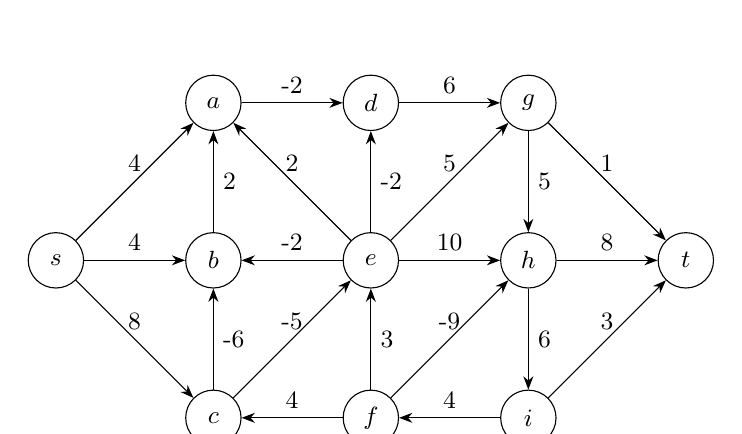
\begin{tikzpicture}[
      mycircle/.style={
         circle,
         draw=black,
         fill=white,
         fill opacity = 0.3,
         text opacity=1,
         inner sep=0pt,
         minimum size=20pt,
         font=\small},
      myarrow/.style={-Stealth},
      node distance=0.6cm and 1.2cm
      ]
      \node[mycircle]  at (-3, 0) (s) {$s$};
      \node[mycircle]  at (-1, 2) (a) {$a$};
      \node[mycircle]  at (1, 2) (d) {$d$};
      \node[mycircle]  at (-1, 0) (b) {$b$};
      \node[mycircle]  at (1, 0) (e) {$e$};
      \node[mycircle]  at (-1, -2) (c) {$c$};
      \node[mycircle]  at (1, -2) (f) {$f$};
      \node[mycircle]  at (3, 2) (g) {$g$};
      \node[mycircle]  at (3, 0) (h) {$h$};
      \node[mycircle]  at (3, -2) (i) {$i$};
      \node[mycircle]  at (5, 0) (t) {$t$};

    \foreach \i/\j/\txt/\p/\pp in {% start node/end node/text/position
      s.45/a.225/4/above/0.5,
      s.00/b.180/4/above/0.5,
      s.315/c.135/8/above/0.5,
      a.00/d.180/-2/above/0.5,
      b.90/a.270/2/right/0.5,
      c.90/b.270/-6/right/0.5,
      c.45/e.225/-5/above/0.5,
      d.0/g.180/6/above/0.5,
      e.135/a.315/2/above/0.5,
      e.180/b.0/-2/above/0.5,
      e.90/d.270/-2/right/0.5,
      e.45/g.225/5/above/0.5,
      e.0/h.180/10/above/0.5,
      f.180/c.0/4/above/0.5,
      f.90/e.270/3/right/0.5,
      f.45/h.225/-9/above/0.5,
      g.270/h.90/5/right/0.5,
      g.315/t.135/1/above/0.5,
      h.00/t.180/8/above/0.5,
      h.270/i.90/6/right/0.5,
      i.180/f.0/4/above/0.5,
      i.45/t.225/3/above/0.5
      }
       \draw [myarrow] (\i) -- node[font=\small,\p,pos=\pp] {\txt} (\j);

    \end{tikzpicture}
    \end{center}
\begin{enumerate}
  \item[(a)] What are the shortest path(s) from $s$ to $t$?

    \begin{table}[H]
    \centering
    \caption{Bellman-Ford}
    \label{tab:simple3col}
    \begin{tabular}{|c|c|c|c|c|c|c|c|c|c|c|c|}   
        \hline
        \textbf{K-edges} & \textbf{s} & \textbf{a} & \textbf{b} & \textbf{c} & \textbf{d} & \textbf{e} & \textbf{f} & \textbf{g} & \textbf{h} & \textbf{i} & \textbf{t}\\
        \hline
        0 & $ \textbf{0} $ & $\infty$ & $\infty$ & $\infty$ & $\infty$ & $\infty$ & $\infty$ & $\infty$ & $\infty$ & $\infty$ & $\infty$\\
        \hline
        1 & $ 0 $ & $\textbf{4}_s$ & $\textbf{4}_s$ & $\textbf{8}_s$ & $\infty$ & $\infty$ & $\infty$ & $\infty$ & $\infty$ & $\infty$ & $\infty$\\
        \hline
        2 & $ 0 $ & $4_s$ & $\textbf{2}_c$ & $8_s$ & $\textbf{2}_a$ & $\textbf{3}_c$ & $\infty$ & $\infty$ & $\infty$ & $\infty$ & $\infty$\\
        \hline
        3 & $ 0 $ & $4_s$ & $\textbf{1}_{e}$ & $8_s$ & $\textbf{1}_e$ & $3_c$ & $\infty$ & $\textbf{8}_{ed}$ & $\textbf{13}_e$ & $\infty$ & $\infty$\\
        \hline
        4 & $ 0 $ & $\textbf{3}_{b}$ & $2_c$ & $8_s$ & $1_e$ & $3_c$ & $\infty$ & $\textbf{7}_{d}$ & $13_e$ & $\textbf{19}_h$ & $\textbf{9}_g$\\
        \hline
        5 & $ 0 $ & $3_b$ & $2_c$ & $8_s$ & $\textbf{1}_{ea}$ & $3_c$ & $\textbf{23}_i$ & $7_{d}$ & $\textbf{12}_g$ & $19_h$ & $\textbf{8}_g$\\
        \hline
        6 & $ 0 $ & $3_b$ & $2_c$ & $8_s$ & $1_e$ & $3_c$ & $23_i$ & $\textbf{7}_{d}$ & $12_g$ & $\textbf{18}_h$ & $8_g$\\
        \hline
        7 & $ 0 $ & $3_b$ & $2_c$ & $8_s$ & $1_e$ & $3_c$ & $\textbf{22}_i$ & $7_{d}$ & $\textbf{12}_g$ & $18_h$ & $\textbf{8}_g$\\
        \hline
        8 & $ 0 $ & $3_b$ & $2_c$ & $8_s$ & $1_e$ & $3_c$ & $22_i$ & $7_{d}$ & $12_g$ & $\textbf{18}_h$ & $8_g$\\
        \hline
    \end{tabular}
    \end{table}

    The shortest paths from $s$ to $t$: 
    \begin{enumerate}
      \item $\textbf{s} \rightarrow \textbf{c} \rightarrow \textbf{e} \rightarrow \textbf{d} \rightarrow \textbf{g} \rightarrow \textbf{t}$
      \item $\textbf{s} \rightarrow \textbf{c} \rightarrow \textbf{e} \rightarrow \textbf{b} \rightarrow \textbf{a} \rightarrow \textbf{d} \rightarrow \textbf{g} \rightarrow \textbf{t}$
    \end{enumerate}


\item[(b)] Bellman-Ford requires no negative cycles. By changing the weight of $e= \{h,i\}$, we create a negative cycle of $f \rightarrow h \rightarrow h \rightarrow i \rightarrow f$. We cannot reliably use Bellman-Ford on this new graph. 

\end{enumerate}

\section*{Problem 2: Road Trip Planning (25 points)}
\begin{enumerate}
\item[(a)] We turn the problem into a graph traversal on a weighted directed graph, and look for the path with the largest happiness value, modeled as edge weights using a modified Bellman-Ford.
  \begin{enumerate}
    \item[]$\textbf{Create graph}$ Start with all $n$ destinations as vertices, $v_i \st i \in \{1, \dots, n\}$, $x = n + 1$ as the ending vertex, $v_{n+1}$, and $x = 0$ as the starting vertex, $v_0$. From each vertex, form directed edges, $e_{i, j}$, to all destinations within $300$ miles of itself without going backwards. Let the weight of those edges, $l_{j}$, represent the happiness value of the destination vertex with $l_{n+1} = 0$.
    
    This is our graph $G(V, E)$ with $n+2$ vertices and $O(n^2)$ edges. There exists no cycles since we cannot go backwards.

    \item[]$\textbf{Subproblem:}$ Let $d_k(i)$ be the maximal length of a walk from $v_0$ to $v_i$ using exactly $k$ edges. For each vertex $v_i \in V(G)$ what is $d_k(i)$?
    \item[]$\textbf{Recurrence Relation:}$ 
    \[d_0(0) = 0; ~d_0(i) = -\infty, ~\forall i \in \{1, \dots, n\}\]
    \[d_k(j) = \max_{v_i \in V(G) \st e_{i,j} \in E(G)} \{d_{k-1}(i) + l_{j}\} \tor -\infty \text{ if the set is empty}\]
    Note that we negate edges that cannot be reached with exactly $k$ edges. 

    \item[]$\textbf{Algorithm:}$ Use a modified Bellman-Ford algorithm with the recurrence relationship as dictated above in order to traverse the graph. We stop at exactly $k+1$ edges and recurse to find the best schedule from $x = 0$ to $x = n+1$ that include exactly $k+1$ edges.

  \end{enumerate}

\item[(b)] Let $P$ be the an optimal walk from node $0$ to node $j$ using exactly $k$ edges. Let $i$ be some predecessor to $j$. Then the path from $0$ to $i$ has exactly $k-1$ edges and therefore has value $\leq d_{k-1}(i)$. Therefore, $P \leq d_{k-1}(i) + l_j$. 

$\Rightarrow P \leq \max_{v_i \in V(G) \st e_{i,j} \in E(G)} \{d_{k-1}(i) + l_{j}\}$

Conversely, for any $i \in V(G) \st e = \{i, j\} \in E(G)$, we can find the optimal walking to achieve $d_{k-1}(i)$. We then append $l_j$ for a $k$ edge walk. All traversals to node $j$ using exactly $k$ edges must first arrive at some node $i$ using exactly $k-1$ edges and then go to node $j$ using one more edge.  Therefore $\{d_{k-1}(i) + l_{j}\}_{v_i \in V(G) \st e_{i,j} \in E(G)}$ gives us all the possible way to traverse to node $j$ using exactly $k$ edges. 

$\Rightarrow d_k(j) \geq \max_{v_i \in V(G) \st e_{i,j} \in E(G)} \{d_{k-1}(i) + l_{j}\}$

\item[(c)] Creating the graph with $n+2$ nodes and iterating through to find valid edges requires $O(n^2)$ time. The modified Bellman-Ford has $ (k+1) * (n+2)$ subproblems. Each subprobelm takes $O(n)$ solve time. Therefore the entire algorithm is $O(kn^2)$
\end{enumerate}

\section*{Problem 3: Lazy Interval Scheduling (30 points)}
\begin{enumerate}
\item[(a)] Incorrect Algorithm. Consider the following set of jobs sorted by \textbf{start time}:
\[ \{[0,2], [3,6], [4,8], [7,16], [9,11], [10,13], [12,14], [15,17]\} \]
and \textbf{end time}: $\{[0,2], [3,6], [4,8], [9,11], [10,13], [12,14], [7,16], [15,17]\}$

By the greedy algorithm, we have the following algorithm progression:
    \begin{table}[h]
    \centering
    \begin{tabular}{|c|c|c|c|}
        \hline
        \textbf{S} & \textbf{t} & \textbf{$[a_i, b_i]$} & \textbf{Looking for $[a_i, b_i]$} \\
        \hline
        $\{\}$ & $0$ & $[0,2]$ & $\msout{[0,2]}, [3,6], [4,8], [9,11], [10,13], [12,14], [7,16], [15,17]$\\
        \hline
        $\{[0,2]\}$ & $2$ & $[3,6]$ & $\msout{[0,2]}, \msout{[3,6]}, [4,8], [9,11], [10,13], [12,14], [7,16], [15,17]$\\
        \hline
        $\{[0,2], [4,8]\}$ & $8$ & $[9,11]$ & $\msout{[0,2]}, \msout{[3,6]}, \msout{[4,8]}, \msout{[9,11]}, [10,13], [12,14], [7,16], [15,17]$\\
        \hline
        $\{[0,2], [4,8], [10,13]\}$ & $13$ & $[15, 17]$ & $\msout{[0,2]}, \msout{[3,6]}, \msout{[4,8]}, \msout{[9,11]}, \msout{[10,13]}, \msout{[12,14]}, \msout{[7,16]}, \msout{[15,17]}$ \\
        \hline
        $\{[0,2], [4,8], [10,13], [15, 17]\}$ & $17$ & DONE & $\msout{[0,2]}, \msout{[3,6]}, \msout{[4,8]}, \msout{[9,11]}, \msout{[10,13]}, \msout{[12,14]}, \msout{[7,16]}, \msout{[15,17]}$ \\
        \hline
    \end{tabular}
    \end{table}
    
    However, evidently the best schedule would be $S = \{[0,2], [3, 6], [7,16]\}$

\item[(b)] We start with the array of all jobs, denoted $A$, sorted by start time.
We define overlap as follows: two jobs $I=[a,b]$ and $J=[a',b']$ overlap iff $a<b'$ or $a'<b$.

\begin{algorithm}[H]
\begin{lstlisting}
Minimize(i):    #i is an index; we recurse on A[i:]
    if i > n-1: return 0

    Jobs = A[i:]
    J = min{job in Jobs: key=job.end}
    Candidates = {job in Jobs : job overlaps J}
    
    best = +infty
    for c in Candidates:    #A is sorted by start time
      k = first index such that A[k].start >= c.end
      best = min(best, w(c) + Minimize(k))
    
    return best
\end{lstlisting}
\end{algorithm}

\textbf{Subproblem:} For each index $i$, what is $\texttt{Minimize}(i)$? we aim to compute $\texttt{Minimize}(0)$. We start with $i=n-1$ and decrement $i$ until $i=0$. Utilizing memoization, each suffix index $i$ is evaluated at most once, so there are $O(n)$ subproblems. 

\textbf{Recurrence Relation}

Assume array of jobs $A$ are sorted by start time, indexed $0, 1, \dots, n-1$. Job $i$ is represented by interval $[a_i,b_i]$ and weight $w(i)$.

Let $F(i)$ denote the minimum total work needed to produce a valid schedule only considering jobs $i,i+1,\dots, n-1 $.

Let $J(i)$ be the index of the job in $\{i,\dots,n-1\}$ with the earliest end time:
\[ J(i) = \min_{k \in \{i,\dots,n-1\}} \{b_k\}\]

Let $C(i)$ be the set of jobs that overlap $J(i)$:
\[C(i) = \{\, x \in \{i,\dots,n-1\}|[a_x,b_x)\cap [a_{J(i)},b_{J(i)}) \neq \emptyset \,\}\]

For any chosen job $x$, let $\text{next}(x)$ be the index of the first job whose start time is at least $b_x$, assume $a_{n} = +\infty$:
\[\text{next}(x) = \min\{\, t \in \{i,\dots,n-1\} | a_t \ge b_x \,\}\]

$\quad$ \underline{Base Case:} $F(n) = 0$

$\quad$  \underline{Recurrence Relation:} $F(i) = \min_{x \in C(i)} ( w_x + F(\text{next}(x)))$
$\nextline$

\textbf{Algorithm}

Once we calculate  $\texttt{Minimize}(0)$, we backtrack to find the optimal schedule, follwing which job within $C(x)$ gives us the minimum $F(x) = w_x + F(next(x))$. 
$\nextline$


\item[(c)] We will prove that this recurrence relation is correct by showing 
\[F(i) = \min_{x \in C(i)} (w_x + F(\text{next}(x)))\]

$F(i)$ is the minimum total work needed to produce a valid schedule using jobs $i,i+1,\dots,n$. $\forall [a_i, b_i] \in C(j), ~a_i < b_{J(i)} \text{ (job $i$ must overlap with job $J(i)$) }\tand b_i > b_{J(i)}$ ($J(i)$ is the job which ends earliest). Therefore $b_{J(i)} - 1 \in [a_i, b_i], ~\forall [a_i, b_i] \in C(j)$ and so all jobs in $C(i)$ overlap each other. We only need to pick one.

By definition, $F(next(x))$ is the minimum workload needed to fill up the time not covered by $[a_i, b_i], ~\forall [a_i, b_i] \in C(j)$. Adding $[a_i, b_i]$ to the schedule determined by backtracking the formation of $F(next(x))$ covers all jobs $i, \dots, n-1$. Therefore, $\{w(x) + F(\text{next}(x))\}_{x \in C(i)}$ produces valid schedules and since $F(i)$ is the the minimum total work to produce a valid schedule...

$\Rightarrow F(i) \leq \min_{x \in C(i)} (w_x + F(\text{next}(x))) \nextline$


We claim that $w_x + F(\text{next}(x)), ~\forall x \in C(i)$ are the only ways to form valid schedules when considering jobs $i, \dots, n-1$ 

We must take a job in $C(i)$, otherwise we have no excuse for not taking job $J(i)$ and we will have to take job $J(i) \in C(i)$ regardless. By definition, $\text{next}(x)$ is the set of jobs not covered by our first choice and $F(\text{next}(x))$ is the minimum workload in order to form a valid schedule which covers all the such jobs. Therefore, these are the minimal valid schedules that cover all jobs $i, i+1, \dots, n-1$

$\Rightarrow F(i) \geq \min_{x \in C(i)} (w_x + F(\text{next}(x)))$

Therefore $F(i) = \min_{x \in C(i)} (w_x + F(\text{next}(x)))$.

\item[(d)] There exists $n$ subproblems and each subproblem takes $O(n)$ time. Therefore we have a time complexity of $O(n^2)$.
\end{enumerate}

\section*{Problem 4: Pok\'{e}mon Battle (25 points)}

\begin{enumerate}
\item[(a)] Let $A$ represent the array of Pok\'{e}mon. For convince, we will use a 1-based index. The Pok\'{e}mon are arranged as specified by the problem such that $A[i] = p_i$.

\textbf{Subproblem:} Who are the possible winners given an interval length of $k$? Let $d_k(i, j)$ represent the set of possible winners between indicies $i$ and $j$ s.t. $i < j \tand j - i + 1= k$. 

\textbf{Algorithm}
\begin{enumerate}
  \item[1)] We start with $k = 1$ and increment until $k = n$.
  \item[2)] Consider some $k$, we iterate through $A$ and create pairings $(i, j)$ s.t. $j - i + 1 = k$. To create unique intervals, it is sufficent to start from some $i$ and set $j = i + k - 1$. We stop creating intervals once the prospective $j > n$ or in other words, $i = n - k + 2$.
  \item[3)]To determine the set of possible winners $d_k(i_o, j_)$, we consider sets $d_{k-1}(i, j)$ s.t. $i \geq i_o \tand j \leq j_o$. Note that there exists exactly two such sets since $k$ is only $1$ larger than $k-1$ so our options are $d_{k-1}(i_o, j-1)$ and $d_{k-1}(i_o + 1, j_o)$.
  \item[] 

\end{enumerate}

\textbf{Recurrence Relation}
\[d_1(i, j) = A[i] = A[j] \text{ (in this case $i$ must be equal to $j$) }\]
\[d_k(i, j) = {}\]



\item[(b)] 10 points: Explain why your algorithm is correct. You do not need to give a rigorous proof.
\item[(c)] 5 points: Analyze the runtime of your algorithm.
\end{enumerate}


\end{document}
